\documentclass[conference]{IEEEtran}
\usepackage[utf8]{inputenc}
\usepackage[T1]{fontenc}
\usepackage{graphicx,booktabs,array,amsmath,xcolor,multirow,url}
\usepackage{cite}
\IfFileExists{spanish.ldf}{\usepackage[spanish,es-noshorthands]{babel}}{}
\AtBeginDocument{%
  \def\tablename{Tabla}\def\figurename{Fig.}\def\abstractname{Resumen}%
  \def\IEEEkeywordsname{Términos de indexación}\def\refname{Referencias}}
\def\BibTeX{{\rm B\kern-.05em{\sc i\kern-.025em b}\kern-.08em T\kern-.1em\lower.7ex\hbox{E}\kern-.125emX}}

\title{Entrenamiento de modelos de Machine Learning para la clasificación de la intención de compra en comercio electrónico}
\author{Jenny Andrea Orozco Osorio, Max Daniel Perez Quintero y Paolo Steven Martinez Cardona\thanks{Los autores pertenecen a la Facultad de Ingeniería, programa de Ingeniería de Sistemas, Universidad de Antioquia, Medellín, Colombia. Correos electrónicos: \{jennya.orozco, mdaniel.perez, paolo.martinez\}@udea.edu.co.}}

\begin{document}
\maketitle

\begin{abstract}
Se aborda la predicción de la intención de compra en sesiones de comercio electrónico como un problema de clasificación binaria supervisada con el \emph{Online Shoppers Purchasing Intention Dataset}, que contiene 12.330 sesiones y una clase positiva de solo 15,5\,\%. Debido a este desbalance, la exactitud por sí sola puede resultar engañosa y no es suficiente para evaluar el desempeño del modelo; por ello se selecciona con exactitud balanceada y se evalúa con el área bajo la curva ROC (ROC-AUC), el F1 de la clase positiva e intervalos de confianza por \emph{bootstrap}. Se comparan ocho modelos (Random Forest, XGBoost, perceptrón multicapa, máquina de vectores de soporte, regresión logística, K vecinos más cercanos, K-Means y mezcla de gaussianas) mediante validación cruzada estratificada de 10 pliegues, con normalización y sobremuestreo SMOTE dentro del \emph{pipeline} para evitar fuga de datos. Se documenta y justifica la codificación de las variables categóricas \texttt{Month}, \texttt{VisitorType} y \texttt{Weekend} mediante un experimento sobre modelos lineales, de distancia y de árboles. Finalmente, se evalúa la reducción de dimensión con análisis de componentes principales (PCA) y UMAP sobre los dos mejores modelos. XGBoost obtuvo el mayor ROC-AUC en prueba (0,931), mientras que PCA y UMAP degradaron el desempeño.
\end{abstract}

\begin{IEEEkeywords}
intención de compra, comercio electrónico, clasificación desbalanceada, SMOTE, codificación de variables, PCA, UMAP.
\end{IEEEkeywords}

\section{Descripción del problema}

\subsection{Contexto y motivación}
Cada visita a una tienda en línea deja registros de navegación, como las páginas consultadas, el tiempo de permanencia y las tasas de rebote y de salida, que permiten caracterizar el comportamiento del visitante \cite{sakar2019}. Sakar et al.\ proponen usar estos datos agregados de la sesión, junto con información del usuario, para predecir en tiempo real si el visitante tiene intención de compra y, combinándolo con la probabilidad de abandono, identificar a quienes conviene abordar para mejorar la conversión \cite{sakar2019}. Un clasificador de intención de compra permite, entonces, priorizar acciones durante la sesión (promociones, recomendaciones o apoyo al usuario) en lugar de analizar el resultado solo después de que la sesión termina.

El objetivo de este trabajo es entrenar y comparar modelos de clasificación binaria que, a partir de las variables de la sesión, determinen si esta termina o no en una compra, evaluándolos con métricas adecuadas para una clase positiva escasa. Además, se estudia si es posible reducir la dimensión del espacio de variables sin perder capacidad predictiva.

\subsection{Composición de la base de datos}
Se utiliza el \emph{Online Shoppers Purchasing Intention Dataset} \cite{uci2018}, con 12.330 sesiones de navegación. Según su documentación, cada sesión corresponde a un usuario distinto dentro de un periodo de un año, de modo que el conjunto no se concentra en una campaña, un día especial o un perfil de usuario \cite{uci2018}. Contiene 18 variables: 17 predictoras (10 numéricas y 7 categóricas) y la variable objetivo \texttt{Revenue}. No presenta datos faltantes, por lo que no requiere imputación. La Tabla~\ref{tab:vars} resume las variables y la codificación adoptada; la justificación de cada decisión se desarrolla en la Sección~\ref{sec:cod}.

Las variables categóricas tienen las siguientes cardinalidades: \texttt{Month}, 10 de los 12 meses del calendario (no hay sesiones de enero ni de abril); \texttt{OperatingSystems}, 8; \texttt{Browser}, 13; \texttt{Region}, 9; \texttt{TrafficType}, 20; \texttt{VisitorType}, 3; y \texttt{Weekend}, 2. Las variables \texttt{OperatingSystems}, \texttt{Browser}, \texttt{Region} y \texttt{TrafficType} están almacenadas como enteros, pero son códigos nominales sin orden.

\begin{table*}[!t]
\centering
\caption{Variables del conjunto de datos y codificación adoptada}
\label{tab:vars}
\small
\begin{tabular}{@{}p{3.0cm}p{2.5cm}p{2.5cm}p{7.4cm}@{}}
\toprule
Variable & Tipo & Codificación & Descripción \\
\midrule
Administrative, Informational, ProductRelated & Numérica entera & Estandarización & Número de páginas administrativas, informativas y de producto visitadas en la sesión. \\
\texttt{*}\_Duration (3 variables) & Numérica continua & Estandarización & Tiempo total (s) en cada tipo de página. \\
BounceRates, ExitRates & Numérica continua & Estandarización & Tasa de rebote y tasa de salida de las páginas visitadas. \\
PageValues & Numérica continua & Estandarización & Valor promedio de una página visitada antes de completar una transacción. \\
SpecialDay & Numérica continua & Estandarización & Cercanía a una fecha especial, entre 0 y 1. \\
Month & Categórica nominal (10 niveles) & One-hot & Mes de la sesión. \\
OperatingSystems, Browser, Region, TrafficType & Categórica nominal (8, 13, 9 y 20 niveles) & One-hot & Códigos del sistema operativo, navegador, región y fuente de tráfico. \\
VisitorType & Categórica nominal (3 niveles) & One-hot & Visitante nuevo, recurrente u otro. \\
Weekend & Binaria & 0/1 & Indica si la sesión ocurrió en fin de semana. \\
Revenue & Binaria & 0/1 & Variable objetivo: la sesión terminó (1) o no (0) en compra. \\
\bottomrule
\end{tabular}
\end{table*}

\subsection{Desbalance de clases}
\label{sec:desb}
La variable objetivo está fuertemente desbalanceada: 10.422 sesiones (84,5\,\%) no terminaron en compra y 1.908 (15,5\,\%) sí lo hicieron, es decir, una razón de desbalance de aproximadamente 5,5 a 1 (una compra por cada 6,5 sesiones). Esto tiene tres consecuencias para el diseño experimental.

Primero, la exactitud por sí sola puede resultar engañosa en presencia de desbalance y no es suficiente para evaluar el desempeño del modelo: un clasificador trivial que siempre prediga ``no compra'' alcanza 84,5\,\% de exactitud con \emph{recall} nulo sobre la clase de interés. La literatura sobre aprendizaje con clases desbalanceadas advierte que la exactitud global por sí sola puede resultar engañosa en este escenario y recomienda métricas por clase y curvas ROC o de precisión--\emph{recall} \cite{he2009}. En particular, la curva de precisión--\emph{recall} resulta más informativa que la ROC cuando la clase positiva es escasa \cite{saito2015}. Por ello se emplea la exactitud balanceada (promedio del \emph{recall} de cada clase) como criterio de selección de hiperparámetros, y el ROC-AUC y el F1 de la clase positiva como métricas sobre el conjunto de prueba, con intervalos de confianza por \emph{bootstrap}.

Segundo, el desbalance obliga a conservar la proporción de clases en todas las particiones: tanto la división entrenamiento/prueba como los pliegues de validación cruzada son estratificados, de modo que cada partición mantiene aproximadamente el 15,5\,\% de compras.

Tercero, se trata el desbalance a nivel de datos con SMOTE, que genera muestras sintéticas de la clase minoritaria interpolando entre vecinos de esa misma clase \cite{chawla2002}. Los estudios previos sobre este conjunto también recurren al sobremuestreo \cite{sakar2019,tanvir2023,alamuri2026}. Como la razón original entre clases es de 0,18 (1.908/10.422), se consideran como valores candidatos razones de sobremuestreo parciales de 0,22, 0,30 y 0,40, utilizando una malla específica según el modelo, en lugar de igualar las clases, con el fin de limitar la proporción de muestras sintéticas. SMOTE se aplica únicamente sobre los datos de entrenamiento de cada pliegue, dentro del \emph{pipeline}, y la evaluación se hace siempre sobre datos con la distribución original.

\subsection{Paradigma de aprendizaje y justificación}
El conjunto de datos contiene una etiqueta conocida para cada sesión (\texttt{Revenue}); por ello el problema se plantea como aprendizaje supervisado, específicamente clasificación binaria con dos resultados posibles: compra y no compra. Se entrenan seis clasificadores supervisados (Random Forest, XGBoost, MLP, SVM, regresión logística y KNN), elegidos por su uso en los trabajos previos sobre este conjunto (Sección~\ref{sec:sota}). Como método de agrupamiento complementario, K-Means forma \emph{clusters} sin utilizar directamente \texttt{Revenue}; posteriormente, cada grupo se asocia con la clase mayoritaria de sus muestras de entrenamiento. Dado que el experimento incluye SMOTE, que utiliza las etiquetas de clase, este procedimiento no constituye una exploración completamente no supervisada. Por su parte, GMM se utiliza como clasificador generativo supervisado: se ajusta una mezcla gaussiana por separado para cada clase y se clasifica mediante la regla de Bayes usando las probabilidades a priori.

\section{Estado del arte}
\label{sec:sota}
Se seleccionaron cuatro trabajos que usan el mismo conjunto de datos, lo que permite comparar no solo los modelos sino también el tratamiento del desbalance, la validación y las métricas (Tabla~\ref{tab:sota}).

Sakar et al.\ compararon Random Forest, SVM y un perceptrón multicapa (MLP), aplicando sobremuestreo y selección de características mediante mRMR; el mejor desempeño correspondió al MLP entrenado con retropropagación resiliente, que con las 6 variables seleccionadas por mRMR alcanzó aproximadamente 87,94\,\% de exactitud y F1 de 0,87 \cite{sakar2019}. Abdullah-All-Tanvir et al.\ ampliaron la comparación a árboles de decisión y XGBoost con una partición 70/30, aplicando SMOTE o submuestreo únicamente al conjunto de entrenamiento y dejando el de prueba con su desbalance original, y reportando también auPR y MCC; XGBoost alcanzó un AUROC de 0,937 y un auPR de 0,754 (con selección de 20 variables y sobremuestreo) y una exactitud de hasta 90,65\,\% \cite{tanvir2023}. Satu e Islam transformaron los datos (min-max, \emph{z-score} y raíz cuadrada), aplicaron SMOTE, eliminación de valores atípicos y selección de características, y evaluaron 14 clasificadores con validación cruzada de 10 pliegues en Weka; Random Forest fue el más estable, con 92,39\,\% de exactitud y F1 de 0,924 (\emph{z-score} y selección por razón de ganancia) y un AUROC de 0,975 (raíz cuadrada y ganancia de información) \cite{satu2023}. Su descripción presenta el balanceo y la selección como pasos sobre el conjunto de datos previos a la clasificación, sin indicar que se ajusten dentro de cada pliegue. Alamuri y Bondalapu integraron SMOTE y selección de características con chi-cuadrado en un \emph{pipeline}, con partición 70/30 estratificada y validación cruzada de 10 pliegues; la SVM con kernel RBF obtuvo el mejor ROC-AUC (0,886) y F1 (0,633), seguida de Random Forest (ROC-AUC 0,882), y las variables más influyentes fueron \texttt{PageValues}, \texttt{ExitRates}, \texttt{ProductRelated\_Duration} y la condición de visitante recurrente \cite{alamuri2026}.

\begin{table*}[!t]
\centering
\caption{Comparación de los trabajos previos sobre el mismo conjunto de datos}
\label{tab:sota}
\footnotesize
\begin{tabular}{@{}p{1.3cm}p{2.7cm}p{2.7cm}p{2.0cm}p{3.2cm}p{3.3cm}@{}}
\toprule
Trabajo & Modelos & Tratamiento del desbalance & Validación & Métricas & Mejor resultado reportado \\
\midrule
\cite{sakar2019} & RF, SVM, MLP & Sobremuestreo y selección de características (mRMR) & --- & Exactitud, F1 & MLP (retropropagación resiliente) con 6 variables seleccionadas por mRMR: aprox. 87,94\,\% exactitud; F1 0,87 \\
\cite{tanvir2023} & SVM, RF, MLP, DT, XGBoost & SMOTE o submuestreo solo en entrenamiento y selección de características & 70/30 & Exactitud, precisión, F1, TPR, TNR, AUROC, auPR, MCC & XGBoost: AUROC 0,937; auPR 0,754; exactitud hasta 90,65\,\% \\
\cite{satu2023} & 14 clasificadores (RF, DT, CART, SMO, LR, \emph{bagging}, entre otros) & SMOTE y eliminación de atípicos (IQR); selección CFS, razón de ganancia y ganancia de información & CV 10 pliegues & Exactitud, precisión, \emph{recall}, F1, AUROC & RF: 92,39\,\% exactitud; F1 0,924; AUROC 0,975 \\
\cite{alamuri2026} & SVC, RF, DT, KNN, NB, Ridge & SMOTE en el \emph{pipeline} y selección chi-cuadrado (6 variables) & 70/30 estratificado y CV 10 pliegues & ROC-AUC, exactitud, precisión, \emph{recall}, F1 & SVC: ROC-AUC 0,886; F1 0,633 \\
\bottomrule
\end{tabular}
\end{table*}

\emph{Síntesis crítica.} Los resultados no son directamente comparables: las particiones (70/30, validación cruzada), el tratamiento del desbalance y las métricas difieren entre estudios. En Tanvir et al.\ el balanceo se aplica únicamente al conjunto de entrenamiento, y Alamuri y Bondalapu integran SMOTE dentro del \emph{pipeline} de validación. La incertidumbre metodológica se limita a Satu e Islam: su descripción presenta el balanceo, la transformación y la selección de características antes de la clasificación, sin aclarar completamente si estos pasos se ajustaron dentro de cada pliegue de validación cruzada. Aplicar sobremuestreo antes de separar entrenamiento y prueba o antes de la división en pliegues puede provocar fuga de información e inflar las métricas. Tres de los cuatro trabajos reportan exactitud como cifra principal, que es poco informativa con 84,5\,\% de clase mayoritaria (Sección~\ref{sec:desb}). En contraste, este trabajo (i) ajusta normalización y SMOTE dentro de cada pliegue, (ii) selecciona hiperparámetros con exactitud balanceada, (iii) evalúa con ROC-AUC y F1 sobre un conjunto de prueba con la distribución original y (iv) reporta intervalos de confianza, lo que acota mejor la incertidumbre de las comparaciones.

\section{Metodología}

\subsection{Partición y validación}
El conjunto se divide en entrenamiento (80\,\%) y prueba (20\,\%) de forma estratificada y con semilla fija. Sobre el entrenamiento se usa validación cruzada estratificada de 10 pliegues (\emph{Stratified K-Fold}), que mantiene la proporción de clases en cada pliegue, y el conjunto de prueba solo se emplea al final. Para cada modelo se construye un \emph{pipeline} con tres etapas: estandarización (\texttt{StandardScaler}), SMOTE y clasificador. Al estar dentro del \emph{pipeline}, el escalamiento y la generación de muestras sintéticas se ajustan solo con el pliegue de entrenamiento, lo que evita fuga de datos hacia el pliegue de validación. La búsqueda de hiperparámetros se hace con \texttt{GridSearchCV} sobre las mallas de la Tabla~\ref{tab:grid}, optimizando la exactitud balanceada.

\subsection{Codificación de variables categóricas}
\label{sec:cod}
La codificación afecta sobre todo a los modelos lineales y basados en distancias (regresión logística, KNN, SVM, MLP, K-Means y GMM), porque una codificación ordinal inadecuada introduce un orden y distancias que los datos no tienen. Para justificar las decisiones se realizó un experimento comparando alternativas con el mismo \emph{split} y con validación cruzada de 5 pliegues únicamente sobre el conjunto de entrenamiento (el de prueba no se usó), con estandarización dentro del \emph{pipeline}.

\textit{Weekend} es binaria y se codifica como 0/1, sin pérdida de información. \textit{VisitorType} es nominal con tres niveles (nuevo, recurrente, otro) y sin orden natural. Una codificación por etiquetas (0, 1, 2) impondría un orden arbitrario, y la diferencia de desempeño entre ambas opciones fue prácticamente nula (Tabla~\ref{tab:cod}); se eligió \emph{one-hot}, que no supone orden y solo añade tres columnas.

\textit{Month} tiene 10 niveles observados dentro de un calendario de 12. Se compararon cuatro alternativas: (a) etiquetas 1--10 por orden de aparición, que fuerzan un orden lineal y comprimen la ausencia de abril (marzo y mayo quedan consecutivos); (b) etiquetas con el número real del mes, que mantienen las distancias del calendario pero tratan el efecto del mes como lineal; (c) codificación cíclica con seno y coseno del número de mes, que respeta la cercanía entre diciembre y enero pero supone un patrón estacional suave; y (d) \emph{one-hot}, que no supone ningún orden ni forma funcional. Adicionalmente se evaluó excluir la variable. Para contexto, un estudio previo codifica \texttt{Month} de forma ordinal (0 a 11) bajo el argumento de preservar la secuencia estacional \cite{alamuri2026}; esa es la alternativa (b), que aquí se contrasta con las demás.

\begin{table}[!t]
\centering
\caption{ROC-AUC en validación cruzada (5 pliegues, solo entrenamiento) según la codificación}
\label{tab:cod}
\footnotesize
\setlength{\tabcolsep}{3pt}
\begin{tabular}{@{}p{3.1cm}cccc@{}}
\toprule
Codificación & RL & KNN & RF & GB \\
\midrule
Month: sin la variable      & 0,8916 & \textbf{0,7568} & 0,9112 & 0,9158 \\
Month: etiquetas 1--10      & 0,8972 & 0,7473 & 0,9238 & 0,9334 \\
Month: etiquetas calendario & 0,8971 & 0,7480 & 0,9238 & 0,9334 \\
Month: seno/coseno          & 0,9001 & 0,7483 & \textbf{0,9265} & 0,9335 \\
Month: \emph{one-hot}       & \textbf{0,9015} & 0,7390 & 0,9249 & \textbf{0,9339} \\
\midrule
VisitorType: \emph{one-hot}$^{*}$ & 0,9001 & 0,7483 & 0,9265 & 0,9335 \\
VisitorType: etiquetas$^{*}$ & 0,9005 & 0,7489 & 0,9275 & 0,9336 \\
\bottomrule
\end{tabular}

\vspace{1mm}
{\footnotesize $^{*}$Con Month en seno/coseno. RL: regresión logística; RF: Random Forest; GB: \emph{gradient boosting} (histograma) como aproximación rápida a XGBoost. Hiperparámetros fijos, sin SMOTE (RL y RF con \texttt{class\_weight} balanceado). Datos: archivo \texttt{online\_shoppers.csv} del repositorio, idéntico al conjunto de UCI (12.330 sesiones, 1.908 compras).}
\end{table}

Los resultados de la Tabla~\ref{tab:cod} muestran que incluir \texttt{Month} mejora el ROC-AUC de la regresión logística, Random Forest y \emph{gradient boosting} respecto a excluirlo, y que \emph{one-hot} es la mejor opción en regresión logística (0,9015) y en \emph{gradient boosting} (0,9339), con seno/coseno prácticamente equivalente. En KNN ocurre lo contrario: la mejor opción es excluir \texttt{Month} (0,7568) y \emph{one-hot} es la peor (0,7390), lo que es coherente con que añadir diez columnas binarias distorsiona las distancias; KNN fue además el modelo de menor desempeño. En Random Forest las diferencias entre codificaciones son pequeñas (0,9238 a 0,9265). Las diferencias entre alternativas son del orden de 0,01 o menores, comparables a la desviación entre pliegues observada en la validación cruzada de los modelos finales (cercana a 0,015 en ROC-AUC), por lo que no deben interpretarse como una ventaja estadística, sino como evidencia de que la elección no deteriora el desempeño de forma relevante. Se adopta \emph{one-hot} para \texttt{Month} porque (i) no impone un orden ni una forma funcional, (ii) fue la mejor en los modelos lineales y de \emph{boosting} y (iii) con 10 niveles el costo es de 10 columnas; la codificación seno/coseno queda como alternativa compacta (2 columnas) con una pérdida de ROC-AUC de 0,0014 en regresión logística, y se reconoce que en KNN, el modelo más sensible a la dimensión, \emph{one-hot} es desfavorable. Con esta codificación, junto con \emph{one-hot} para \texttt{OperatingSystems}, \texttt{Browser}, \texttt{Region}, \texttt{TrafficType} y \texttt{VisitorType}, el espacio de entrada queda en 74 variables.

\subsection{Modelos y mallas de hiperparámetros}
La Tabla~\ref{tab:grid} resume los hiperparámetros explorados. Las razones de SMOTE exploradas se definieron según la malla específica de cada modelo, como se resume en la Tabla~\ref{tab:grid}. En Random Forest, XGBoost, regresión logística, KNN y K-Means se consideraron las razones 0,22, 0,30 y 0,40, mientras que en MLP, SVM y GMM se utilizó una malla más reducida. En Random Forest se empleó además \texttt{class\_weight} balanceado. Se emplean 200 árboles en RF y XGBoost, y en el MLP un máximo de 1.000 iteraciones.

\begin{table}[!t]
\centering
\caption{Malla de hiperparámetros por modelo (SMOTE: razón 0,22/0,30/0,40 y $k$ vecinos 3/5/7 salvo donde se indica)}
\label{tab:grid}
\footnotesize
\begin{tabular}{@{}p{1.3cm}p{6.6cm}@{}}
\toprule
Modelo & Hiperparámetros explorados \\
\midrule
RF & profundidad {10, 20}; \texttt{min\_samples\_leaf} {1, 4}; \texttt{max\_features} = sqrt \\
XGBoost & profundidad {3, 6}; tasa de aprendizaje {0,05, 0,10}; \texttt{subsample} = \texttt{colsample} = 0,8 \\
MLP & capa oculta {(50), (100)}; ReLU; $\alpha$ {$10^{-4}$, $10^{-3}$}; tasa inicial {0,001, 0,01}; SMOTE 0,22/0,30, $k=5$ \\
SVM & núcleo lineal o RBF; $C$ {0,01, 0,1, 1}; $\gamma$ (RBF) {scale, auto, 0,01, 0,1}; SMOTE 0,22/0,30 \\
RL & $C$ {0,01, 0,1, 1, 10}; penalización L2; solver lbfgs; $k$ {3, 5} \\
KNN & $k$ {3, 5, 11}; pesos {uniforme, distancia}; métrica {euclídea, Manhattan}; SMOTE $k=5$ \\
K-Means & \emph{clusters} {2, 3, 4, 5} \\
GMM & componentes {1--4}; covarianza {full, diag, tied, spherical}; iteraciones {100, 200}; inicializaciones {1, 2}; 4 métodos de inicialización; SMOTE 0,22/0,30 \\
\bottomrule
\end{tabular}
\end{table}

\subsection{Métricas de evaluación}
La selección de hiperparámetros usa exactitud balanceada. Sobre el conjunto de prueba se calculan ROC-AUC, F1 de la clase positiva, precisión y \emph{recall} por clase y la matriz de confusión normalizada. Los intervalos de confianza del 95\,\% se obtienen por \emph{bootstrap} con 1.000 remuestreos del conjunto de prueba. Para el modelo con mejor desempeño se analiza además la curva de aprendizaje.

\section{Resultados del entrenamiento}
La Tabla~\ref{tab:best} presenta la mejor combinación de hiperparámetros por modelo y la Tabla~\ref{tab:res} el desempeño en validación cruzada y en prueba.

\begin{table}[!t]
\centering
\caption{Mejor combinación de hiperparámetros por modelo}
\label{tab:best}
\footnotesize
\begin{tabular}{@{}p{1.3cm}p{6.6cm}@{}}
\toprule
Modelo & Hiperparámetros (incluye SMOTE: razón, $k$) \\
\midrule
RF & profundidad 10; \texttt{min\_samples\_leaf} 4; 200 árboles; sqrt; SMOTE 0,22, $k=7$ \\
XGBoost & profundidad 3; tasa 0,05; 200 árboles; \texttt{subsample} 0,8; \texttt{colsample} 0,8; SMOTE 0,40, $k=3$ \\
MLP & una capa oculta de 50 neuronas; ReLU; $\alpha=10^{-3}$; tasa inicial 0,001; SMOTE 0,30, $k=5$ \\
SVM & núcleo lineal; $C=1$; SMOTE 0,30, $k=5$ \\
RL & $C=1$; L2; lbfgs; SMOTE 0,40, $k=3$ \\
KNN & $k=11$; pesos por distancia; métrica euclídea; SMOTE 0,40, $k=5$ \\
K-Means & 4 \emph{clusters}; SMOTE 0,40, $k=7$ \\
GMM & 2 componentes por clase; covarianza esférica; inicialización aleatoria; 100 iteraciones; 2 inicializaciones; SMOTE 0,30, $k=5$ \\
\bottomrule
\end{tabular}
\end{table}

\begin{table*}[!t]
\centering
\caption{Desempeño de los modelos. EB: exactitud balanceada (entrenamiento y validación cruzada de 10 pliegues, media $\pm$ desviación); AUC: ROC-AUC; auPR: área bajo la curva precisión--\emph{recall}; Prec. y Rec.: precisión y \emph{recall} de la clase compra en prueba con umbral 0,5. Prueba: IC 95\,\% por \emph{bootstrap}}
\label{tab:res}
\scriptsize
\setlength{\tabcolsep}{3.5pt}
\begin{tabular}{@{}lcccccccc@{}}
\toprule
Modelo & EB entren. & EB CV & AUC CV & AUC prueba [IC] & auPR prueba & F1 prueba [IC] & Prec. & Rec. \\
\midrule
Random Forest & 0.8872 & 0.8552 $\pm$ 0.0134 & 0.9240 $\pm$ 0.0112 & 0.9127 [0.8974; 0.9271] & 0.6870 & 0.6444 [0.6075; 0.6771] & 0.5355 & 0.8089 \\
XGBoost & 0.8360 & 0.8203 $\pm$ 0.0180 & 0.9340 $\pm$ 0.0077 & \textbf{0.9308} [0.9190; 0.9420] & \textbf{0.7405} & \textbf{0.6753} [0.6354; 0.7107] & 0.6650 & 0.6859 \\
MLP & 0.9533 & 0.7506 $\pm$ 0.0207 & 0.8529 $\pm$ 0.0186 & 0.8458 [0.8233; 0.8662] & 0.5637 & 0.5459 [0.5015; 0.5865] & 0.5642 & 0.5288 \\
SVM (lineal) & 0.7509 & 0.7479 $\pm$ 0.0208 & 0.8989 $\pm$ 0.0099 & 0.8905 [0.8715; 0.9087] & 0.6241 & 0.5723 [0.5254; 0.6163] & 0.6644 & 0.5026 \\
Reg. logística & 0.7649 & 0.7599 $\pm$ 0.0227 & 0.8971 $\pm$ 0.0127 & 0.8852 [0.8667; 0.9041] & 0.6217 & 0.6169 [0.5731; 0.6597] & 0.6825 & 0.5628 \\
KNN & 1.0000 & 0.6537 $\pm$ 0.0190 & 0.7488 $\pm$ 0.0201 & 0.7475 [0.7192; 0.7747] & 0.4000 & 0.4185 [0.3753; 0.4617] & 0.4236 & 0.4136 \\
K-Means & 0.5000 & 0.5003 $\pm$ 0.0010 & 0.5031 $\pm$ 0.0094 & 0.5000 [0.5000; 0.5000] & 0.1549 & 0.0000 [0.0000; 0.0000] & 0.0000 & 0.0000 \\
GMM & 0.7091 & 0.7221 $\pm$ 0.0284 & 0.8114 $\pm$ 0.0282 & 0.7772 [0.7508; 0.8015] & 0.3688 & 0.4503 [0.4152; 0.4882] & 0.3439 & 0.6518 \\
\bottomrule
\end{tabular}
\end{table*}

XGBoost presentó el mejor desempeño general entre los modelos evaluados, con un ROC-AUC de 0.9308 y un auPR de 0.7405 en el conjunto de prueba. También obtuvo el mayor F1, con 0.6753, y mantuvo un equilibrio entre precisión y sensibilidad, con valores de 0.6650 y 0.6859, respectivamente. Random Forest alcanzó un ROC-AUC de 0.9127 y un F1 de 0.6444. Aunque su precisión fue menor, con 0.5355, obtuvo la sensibilidad más alta entre los principales clasificadores, con 0.8089, por lo que identificó una mayor proporción de las sesiones que terminaron en compra.

Los modelos lineales mostraron un desempeño competitivo, aunque inferior al de los modelos basados en árboles. SVM alcanzó un ROC-AUC de 0.8905 y la regresión logística obtuvo 0.8852. MLP presentó un ROC-AUC de 0.8458, mientras que KNN descendió hasta 0.7475. GMM obtuvo un ROC-AUC de 0.7772 y un recall de 0.6518, aunque con una precisión de 0.3439. K-Means no consiguió separar adecuadamente las clases y presentó un ROC-AUC de 0.5000, equivalente al comportamiento esperado de un clasificador sin capacidad discriminativa.

La razón de SMOTE seleccionada fue 0,40 en cuatro modelos (XGBoost, regresión logística, KNN y K-Means), 0,30 en tres (MLP, SVM y GMM) y 0,22 en uno (Random Forest). Como 0,40 es el límite superior de la malla, no puede descartarse que razones mayores mejoren esos modelos. La curva de aprendizaje de XGBoost (Fig.~\ref{fig:curva}) muestra que el ROC-AUC de validación se estabiliza cerca de 0,934 con más de 6.000 muestras, mientras que el de entrenamiento baja hasta 0,946; la brecha final, inferior a 0,015, indica un sobreajuste moderado y que más datos aportarían poco. La matriz de confusión de XGBoost muestra que el modelo mantiene una alta capacidad para reconocer las sesiones que no finalizan en compra y logra identificar aproximadamente el 68.6\,\% de las sesiones que sí terminan en compra. Esto implica que cerca del 31.4\,\% de los compradores reales permanece clasificado como no comprador. El resultado refleja el compromiso existente entre reducir los falsos positivos y conservar una sensibilidad suficiente frente a la clase minoritaria.

\begin{figure}[!t]
\centering
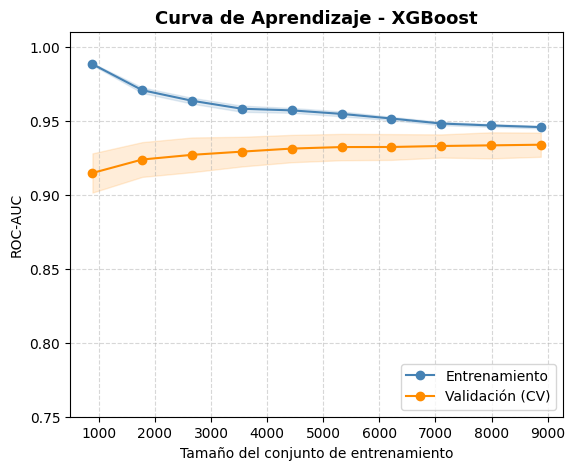
\includegraphics[width=0.85\columnwidth]{figuras/fig_xgb_learning.png}
\caption{Curva de aprendizaje de XGBoost (ROC-AUC, validación cruzada)}
\label{fig:curva}
\end{figure}

\begin{figure}[!t]
\centering
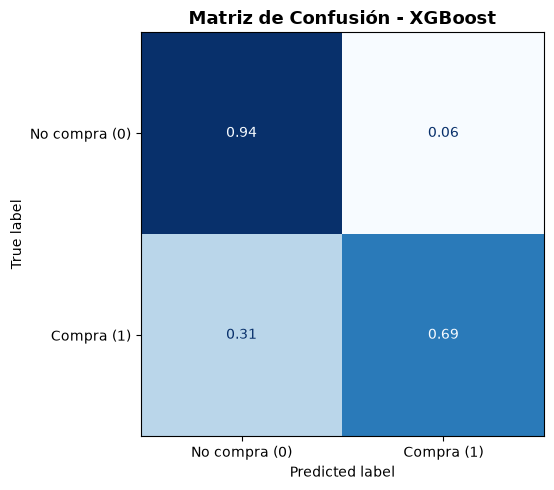
\includegraphics[width=0.75\columnwidth]{figuras/fig_xgb_confusion.png}
\caption{Matriz de confusión normalizada de XGBoost en el conjunto de prueba}
\label{fig:conf}
\end{figure}

\section{Reducción de dimensión}
Se evalúa si es posible reducir la complejidad del sistema sin perder capacidad predictiva, aplicando PCA y UMAP sobre los dos modelos con mejor desempeño (Random Forest y XGBoost), usando los hiperparámetros de la Tabla~\ref{tab:best}.

\subsection{Análisis individual de variables}
Se calculó, para cada variable, la correlación absoluta de Pearson con \texttt{Revenue} y el \emph{Information Value} (IV), discretizando las variables continuas en cuantiles. El IV se interpretó con la escala usual: menor de 0,02, nulo; 0,02--0,1, débil; 0,1--0,3, medio; mayor o igual a 0,3, fuerte. Se consideran candidatas a eliminación las variables con $|r|<0{,}05$ e IV $<0{,}02$ simultáneamente; no se eliminan directamente porque los modelos de árboles pueden aprovechar relaciones no lineales que el análisis univariado no captura.

\texttt{PageValues} es, con amplia diferencia, la variable más discriminativa (IV = 2,43), seguida de \texttt{ExitRates} (0,86), \texttt{BounceRates} (0,52), \texttt{ProductRelated\_Duration} (0,50) y \texttt{ProductRelated} (0,42), todas con IV fuerte. Con IV medio aparecen \texttt{Administrative\_Duration} (0,24), \texttt{Administrative} (0,16), \texttt{Month\_Nov} (0,14), \texttt{TrafficType\_2} (0,12) y \texttt{SpecialDay} (0,11); las categorías de \texttt{VisitorType} tienen IV débil (0,07). Esto es coherente con la importancia de \texttt{PageValues} y \texttt{ProductRelated\_Duration} señalada en \cite{alamuri2026}, que seleccionó \texttt{PageValues}, \texttt{ExitRates}, \texttt{ProductRelated\_Duration} y \texttt{BounceRates} entre sus seis variables principales. Según Pearson, \texttt{PageValues} también es la más asociada con \texttt{Revenue} ($|r|=0{,}50$), seguida de \texttt{ExitRates} (0,21), \texttt{ProductRelated} (0,16), \texttt{BounceRates} (0,15), \texttt{ProductRelated\_Duration} (0,15) y \texttt{Month\_Nov} (0,15); el resto de las variables tiene $|r|<0{,}15$, en su mayoría por debajo de 0,05 (por ejemplo, las categorías de \texttt{Region} y \texttt{Browser}), lo que es esperable en variables nominales codificadas como indicadoras. Con ambos criterios resultan 51 candidatas a eliminación, todas indicadoras de variables nominales: las 13 categorías de \texttt{Browser}, las 9 de \texttt{Region}, 15 de \texttt{TrafficType}, 6 de \texttt{OperatingSystems}, 6 de \texttt{Month} (agosto, julio, junio, septiembre, octubre y diciembre), \texttt{VisitorType\_Other} y \texttt{Weekend}. Como se indicó, no se eliminan: son categorías individuales de variables que en conjunto pueden aportar, y los modelos de árboles las manejan sin penalización.

\subsection{Extracción de características}
\emph{PCA.} Los datos se estandarizan y se conservan los componentes necesarios para explicar al menos el 95\,\% de la varianza acumulada. El orden del \emph{pipeline} es: estandarización, PCA, SMOTE y clasificador, de modo que cada transformación se ajusta solo con el pliegue de entrenamiento. Se requirieron 57 componentes de las 74 variables (reducción de 23,0\,\%). \emph{UMAP.} Se evaluaron 2, 5, 10, 15 y 20 componentes y se eligió el que maximiza el ROC-AUC promedio en validación cruzada de ambos modelos, que resultó ser 2 (reducción de 97,3\,\%); el \emph{pipeline} es estandarización, UMAP, SMOTE y clasificador.

\begin{table}[!t]
\centering
\caption{Modelos base frente a PCA y UMAP}
\label{tab:red}
\footnotesize
\setlength{\tabcolsep}{0.5pt}
\begin{tabular}{@{}lcccccc@{}}
\toprule
Modelo & AUC CV & AUC prueba & auPR & F1 & Dim. & Reduc. \\
\midrule
RF base & 0.9240 $\pm$ 0.0112 & 0.9127 & 0.6870 & 0.6444 & 74 & 0\,\% \\
RF + PCA & 0.8645 $\pm$ 0.0198 & 0.8435 & 0.5624 & 0.5261 & 57 & 23.0\,\% \\
RF + UMAP & 0.5583 $\pm$ 0.0302 & 0.5942 & 0.2774 & 0.2450 & 2 & 97.3\,\% \\
XGBoost base & 0.9340 $\pm$ 0.0077 & 0.9308 & 0.7405 & 0.6753 & 74 & 0\,\% \\
XGBoost + PCA & 0.8749 $\pm$ 0.0184 & 0.8580 & 0.5913 & 0.5532 & 57 & 23.0\,\% \\
XGBoost + UMAP & 0.5715 $\pm$ 0.0361 & 0.5980 & 0.2826 & 0.2321 & 2 & 97.3\,\% \\
\bottomrule
\end{tabular}
\end{table}

Con el criterio de varianza acumulada igual o superior al 95\,\%, PCA conservó 57 componentes de las 74 variables originales, lo que representa una reducción del 23.0\,\%. Sin embargo, esta reducción produjo una disminución clara del desempeño. En Random Forest, el ROC-AUC en prueba pasó de 0.9127 a 0.8435, mientras que en XGBoost descendió de 0.9308 a 0.8580.

La reducción mediante UMAP fue considerablemente mayor, al representar las 74 variables mediante dos componentes. No obstante, el desempeño disminuyó de forma más pronunciada. Random Forest obtuvo un ROC-AUC de 0.5942 y XGBoost de 0.5980. Estos resultados indican que, para este problema, la compresión de la información mediante PCA o UMAP elimina parte de la estructura discriminativa que utilizan los clasificadores. Por esta razón, se conservaron las 74 variables del espacio original.

\section{Discusión}
Los ROC-AUC en prueba de XGBoost (0.9308) y Random Forest (0.9127) son cercanos al AUROC de 0,937 y al auPR de 0,754 reportados con XGBoost por \cite{tanvir2023} (aquí, 0.7405 de auPR) y superiores a los de \cite{alamuri2026} (ROC-AUC de 0,886 con SVM y 0,882 con Random Forest) y algo inferiores a los de \cite{satu2023} (AUROC de 0,975 con Random Forest). Las diferencias pueden asociarse a las particiones usadas (70/30 o validación cruzada) y al tratamiento del sobremuestreo: en \cite{tanvir2023} se aplica solo al entrenamiento, mientras que en \cite{satu2023} el balanceo, la transformación y la selección se describen como pasos sobre el conjunto de datos antes de la validación cruzada, un procedimiento que, si no se ajusta dentro de cada pliegue, puede favorecer las métricas; aquí el preprocesamiento se ajusta dentro de cada pliegue, una estimación más conservadora. Con la información disponible no es posible atribuir la diferencia a una sola causa, y las métricas de umbral (F1, precisión, \emph{recall}) no son comparables directamente con las de esos estudios.

Los ensambles de árboles superan a los modelos lineales, a los basados en distancias y a las redes (Tabla~\ref{tab:res}). La brecha entre entrenamiento y validación del MLP y de KNN indica sobreajuste, que en KNN puede agravarse por la distancia en un espacio de 74 variables, la mayoría binarias. La caída de desempeño con PCA y UMAP sugiere que la información discriminativa no se concentra en pocas direcciones de alta varianza. Como limitaciones, la razón de SMOTE óptima quedó en el borde de la malla en cuatro modelos y la comparación entre XGBoost y Random Forest no incluye una prueba estadística pareada.

\section{Conclusiones}
\begin{enumerate}
\item El problema presenta un desbalance de 5,5 a 1, por lo que la exactitud por sí sola puede resultar engañosa y no es suficiente para evaluar el desempeño del modelo; la selección con exactitud balanceada y la evaluación con ROC-AUC, auPR, F1 e intervalos de confianza dan una comparación más informativa.
\item La codificación \emph{one-hot} de \texttt{Month} y de \texttt{VisitorType} no deteriora el desempeño frente a las alternativas probadas, y excluir \texttt{Month} reduce el ROC-AUC en regresión logística, Random Forest y \emph{gradient boosting} (no en KNN); las diferencias entre codificaciones son comparables a la variabilidad entre pliegues.
\item Entre los modelos evaluados, XGBoost presentó el mejor desempeño general, con un ROC-AUC de 0.9308, un auPR de 0.7405 y un F1 de 0.6753 en el conjunto de prueba. Random Forest obtuvo un ROC-AUC de 0.9127 y alcanzó el mayor recall entre los modelos principales, con 0.8089, aunque con una precisión menor de 0.5355. Estos resultados muestran dos comportamientos diferentes: XGBoost ofrece un mejor equilibrio global entre las métricas, mientras que Random Forest favorece la detección de una mayor proporción de compradores.
\item \texttt{PageValues} es la variable más discriminativa (IV = 2,43), seguida de \texttt{ExitRates}, \texttt{BounceRates} y las variables de páginas de producto.
\item La reducción de dimensionalidad no produjo mejoras frente al espacio original. PCA conservó 57 componentes y redujo el ROC-AUC a 0.8435 en Random Forest y 0.8580 en XGBoost. UMAP, utilizando dos componentes, obtuvo valores de 0.5942 y 0.5980, respectivamente. Por lo tanto, para los modelos evaluados, conservar las 74 variables originales permitió mantener una mayor capacidad discriminativa.
\end{enumerate}

\begin{thebibliography}{00}
\bibitem{sakar2019}
C. O. Sakar, S. O. Polat, M. Katircioglu, and Y. Kastro, ``Real-time prediction of online shoppers' purchasing intention using multilayer perceptron and LSTM recurrent neural networks,'' \emph{Neural Comput. Appl.}, vol. 31, no. 10, pp. 6893--6908, Oct. 2019, doi: 10.1007/s00521-018-3523-0.

\bibitem{uci2018}
C. O. Sakar and Y. Kastro, ``Online shoppers purchasing intention dataset,'' UCI Machine Learning Repository, 2018. [Online]. Available: https://doi.org/10.24432/C5F88Q

\bibitem{he2009}
H. He and E. A. Garcia, ``Learning from imbalanced data,'' \emph{IEEE Trans. Knowl. Data Eng.}, vol. 21, no. 9, pp. 1263--1284, Sep. 2009.

\bibitem{saito2015}
T. Saito and M. Rehmsmeier, ``The precision-recall plot is more informative than the ROC plot when evaluating binary classifiers on imbalanced datasets,'' \emph{PLoS ONE}, vol. 10, no. 3, Art. no. e0118432, 2015.

\bibitem{chawla2002}
N. V. Chawla, K. W. Bowyer, L. O. Hall, and W. P. Kegelmeyer, ``SMOTE: Synthetic minority over-sampling technique,'' \emph{J. Artif. Intell. Res.}, vol. 16, pp. 321--357, 2002.

\bibitem{tanvir2023}
A.-A. Tanvir, I. A. Khandokar, A. K. M. Islam, S. Islam, and S. Shatabda, ``A gradient boosting classifier for purchase intention prediction of online shoppers,'' \emph{Heliyon}, vol. 9, no. 4, Art. no. e15163, 2023, doi: 10.1016/j.heliyon.2023.e15163.

\bibitem{satu2023}
M. S. Satu and S. F. Islam, ``Modeling online customer purchase intention behavior applying different feature engineering and classification techniques,'' \emph{Discov. Artif. Intell.}, vol. 3, Art. no. 36, 2023, doi: 10.1007/s44163-023-00086-0.

\bibitem{alamuri2026}
O. R. S. G. Alamuri and C. K. Bondalapu, ``Predicting e-commerce purchase intention using machine learning,'' \emph{ASEAN J. Sci. Technol. Rep.}, vol. 29, no. 1, Art. no. e260159, 2026, doi: 10.55164/ajstr.v29i1.260159.
\end{thebibliography}
\end{document}
